\chapter{Speech and Person Recognition in detail}
\label{chap:robogame-appendix}

\section{Questions for Speech and Person Recognition}
The questions the robot must answer in the RoboGame test are taken from a small set of predefined trivia questions including information about the arena, the crowd, the list of predefined objects, and the robot's environment.

A generator is publicly available at https://github.com/kyordhel/GPSRCmdGen. The official SPR Command Generator and the official grammars will be made available two months before the competition. However, teams must be aware that the categories, objects and other data is provided for testing purposes only and will adapt to the environment during the setup days. 

\subsection{Question distribution}
The questions to be asked in both, the \textit{riddle game} and the \textit{blind man's bluff game} tasks, are distributed in the following proportion:
\begin{itemize}
    \item One is a predefined question
    \item Between one and two are about the arena and its status
    \item Between one and two are about the crowd
    \item Between one and two are about the list of official objects
\end{itemize}
However, it is important to remark that \textbf{questions won't be asked in any specific order}. This is since the robot must be able to answer any type of question at any given time. For instance, the robot may be asked first about the arena, then about object, later on a predefined question, and finally about the crowd.

\subsection{Arena Questions}
The arena-questions are a set of queries about the features of the RoboCup@Home Arena itself, including its furniture and configuration (e.g. rooms and locations). The arena is considered to be in its normal state and the robot must answer accordingly, without needing to move and verify the state.

Some example arena-questions are:
\begin{enumerate}
    \item Where is the shelf? $\rightarrow$ \textit{The shelf is in the kitchen}
    \item Where is the plant? $\rightarrow$ \textit{The plant is in the living room}
    \item How many chairs are in the dining room? $\rightarrow$ \textit{There are six chairs in the dining room}
\end{enumerate}

\subsection{Crowd \& Operator Questions}
The crowd-questions are a set of queries about the features of the crowd the robot observed at the very beginning of the test.

Some example crowd-questions are:
\begin{enumerate}
    \item Size of the crowd
    \item Number of children
    \item Number of male or female people
    \item Number of people waiving or rising arms
    \item Number of people standing, sitting or lying
    \item How old do you think I am? $\rightarrow$ \textit{I think you are 23 years old}.
    \item The sitting person was a man or woman? $\rightarrow$ \textit{The sitting person was a man}.
    \item Am I a man or a woman? $\rightarrow$ \textit{I couldn't tell.}
\end{enumerate}

\subsection{Object Questions}
The object-questions are built on basis of the features of the predefined objects used during the competition and their categories. Such features include color, shape, size, type, weight, category, predefined location, etc. The arena is considered to be in its normal state and the robot must answer accordingly, without needing to move and verify the state.

Some example object-questions are:
\begin{enumerate}
    \item What's the smallest food? $\rightarrow$ \textit{The egg is the smallest in the food category}.
    \item What's the lightest drink? $\rightarrow$ \textit{The Coke Zero, is lighter than water}.
    \item Where can I find the tray? $\rightarrow$ \textit{The tray is in the shelf}.
    \item Where can I find the beer? $\rightarrow$ \textit{I put it into the fridge for you, master}.
    \item What's the color of the shampoo? $\rightarrow$ \textit{The shampoo is blue}.
    \item What's the color of the sponge? $\rightarrow$ \textit{The sponge is yellow and has square pants}.
    \item What objects are in the closet? $\rightarrow$ \textit{The shampoo, soap, the sponge and a cloth}.
    \item How many objects are in the shelf? $\rightarrow$ \textit{There are five objects in the shelf}.
    \item Do the objects in the cupboard belong to the same category? $\rightarrow$ \textit{Yes. They are all food}.
    % %%% For the next year, maybe %%% %
    % \item What objects are in the closet? $\rightarrow$ \textit{The shampoo, soap, the sponge and a cloth}.
    % \item How many are they? $\rightarrow$ \textit{There are four objects in the closet}.
    % \item Do they belong to the same category? $\rightarrow$ \textit{They are all cleaning stuff}.
\end{enumerate}

Please note that some questions may refer to a previous question or answer. 

\subsubsection{Predefined Questions}
In addition to the other questions, 10 predefined trivia-questions will be announced during the setup days.

Some example predefined-questions are:
\begin{enumerate}
    \item What day is today?
    \item What is your name?
    \item What is your team's name?
    \item What time is it?
    \item In which year was RoboCup@Home founded?
    \item What was the last question?
\end{enumerate}

Please note that some questions may refer to a previous question or answer. 

\section{People setup in \textit{blind man's bluff game}}
People in the \textit{blind man's bluff game} is arranged by the referees in random fashion, but considering each league's robot capabilities. In every turn, the referee chooses which person will ask the next question. This person can be the same one who asked a question in the previous turn; but no chosen person can be in front of the robot.

\textbf{Standing \textit{in front of} the robot:} A person is considered to be standing \textit{in front of} the robot when is located in the cone of approximately $60^{\circ}$ (approximated range of $\big[-\frac{\pi}{6}, \frac{\pi}{6}\big]$, with zero facing forward) which middle is aligned (and facing) whatever part of the robot that functionally operates as front or face for Human-Robot interaction purposes, and with center in the before mentioned central part of the robot.

\textbf{Standing \textit{behind} the robot:} A person is considered to be standing \textit{behind} the robot when is located in the cone of approximately $60^{\circ}$ (approximated range of $\big[\frac{5\pi}{6}, \frac{7\pi}{6}\big]$, with zero facing forward) which is in direct opposition, i.e. mirrors, the front of the robot described in the preceding paragraph.

\begin{figure}[H]
    \begin{center}
        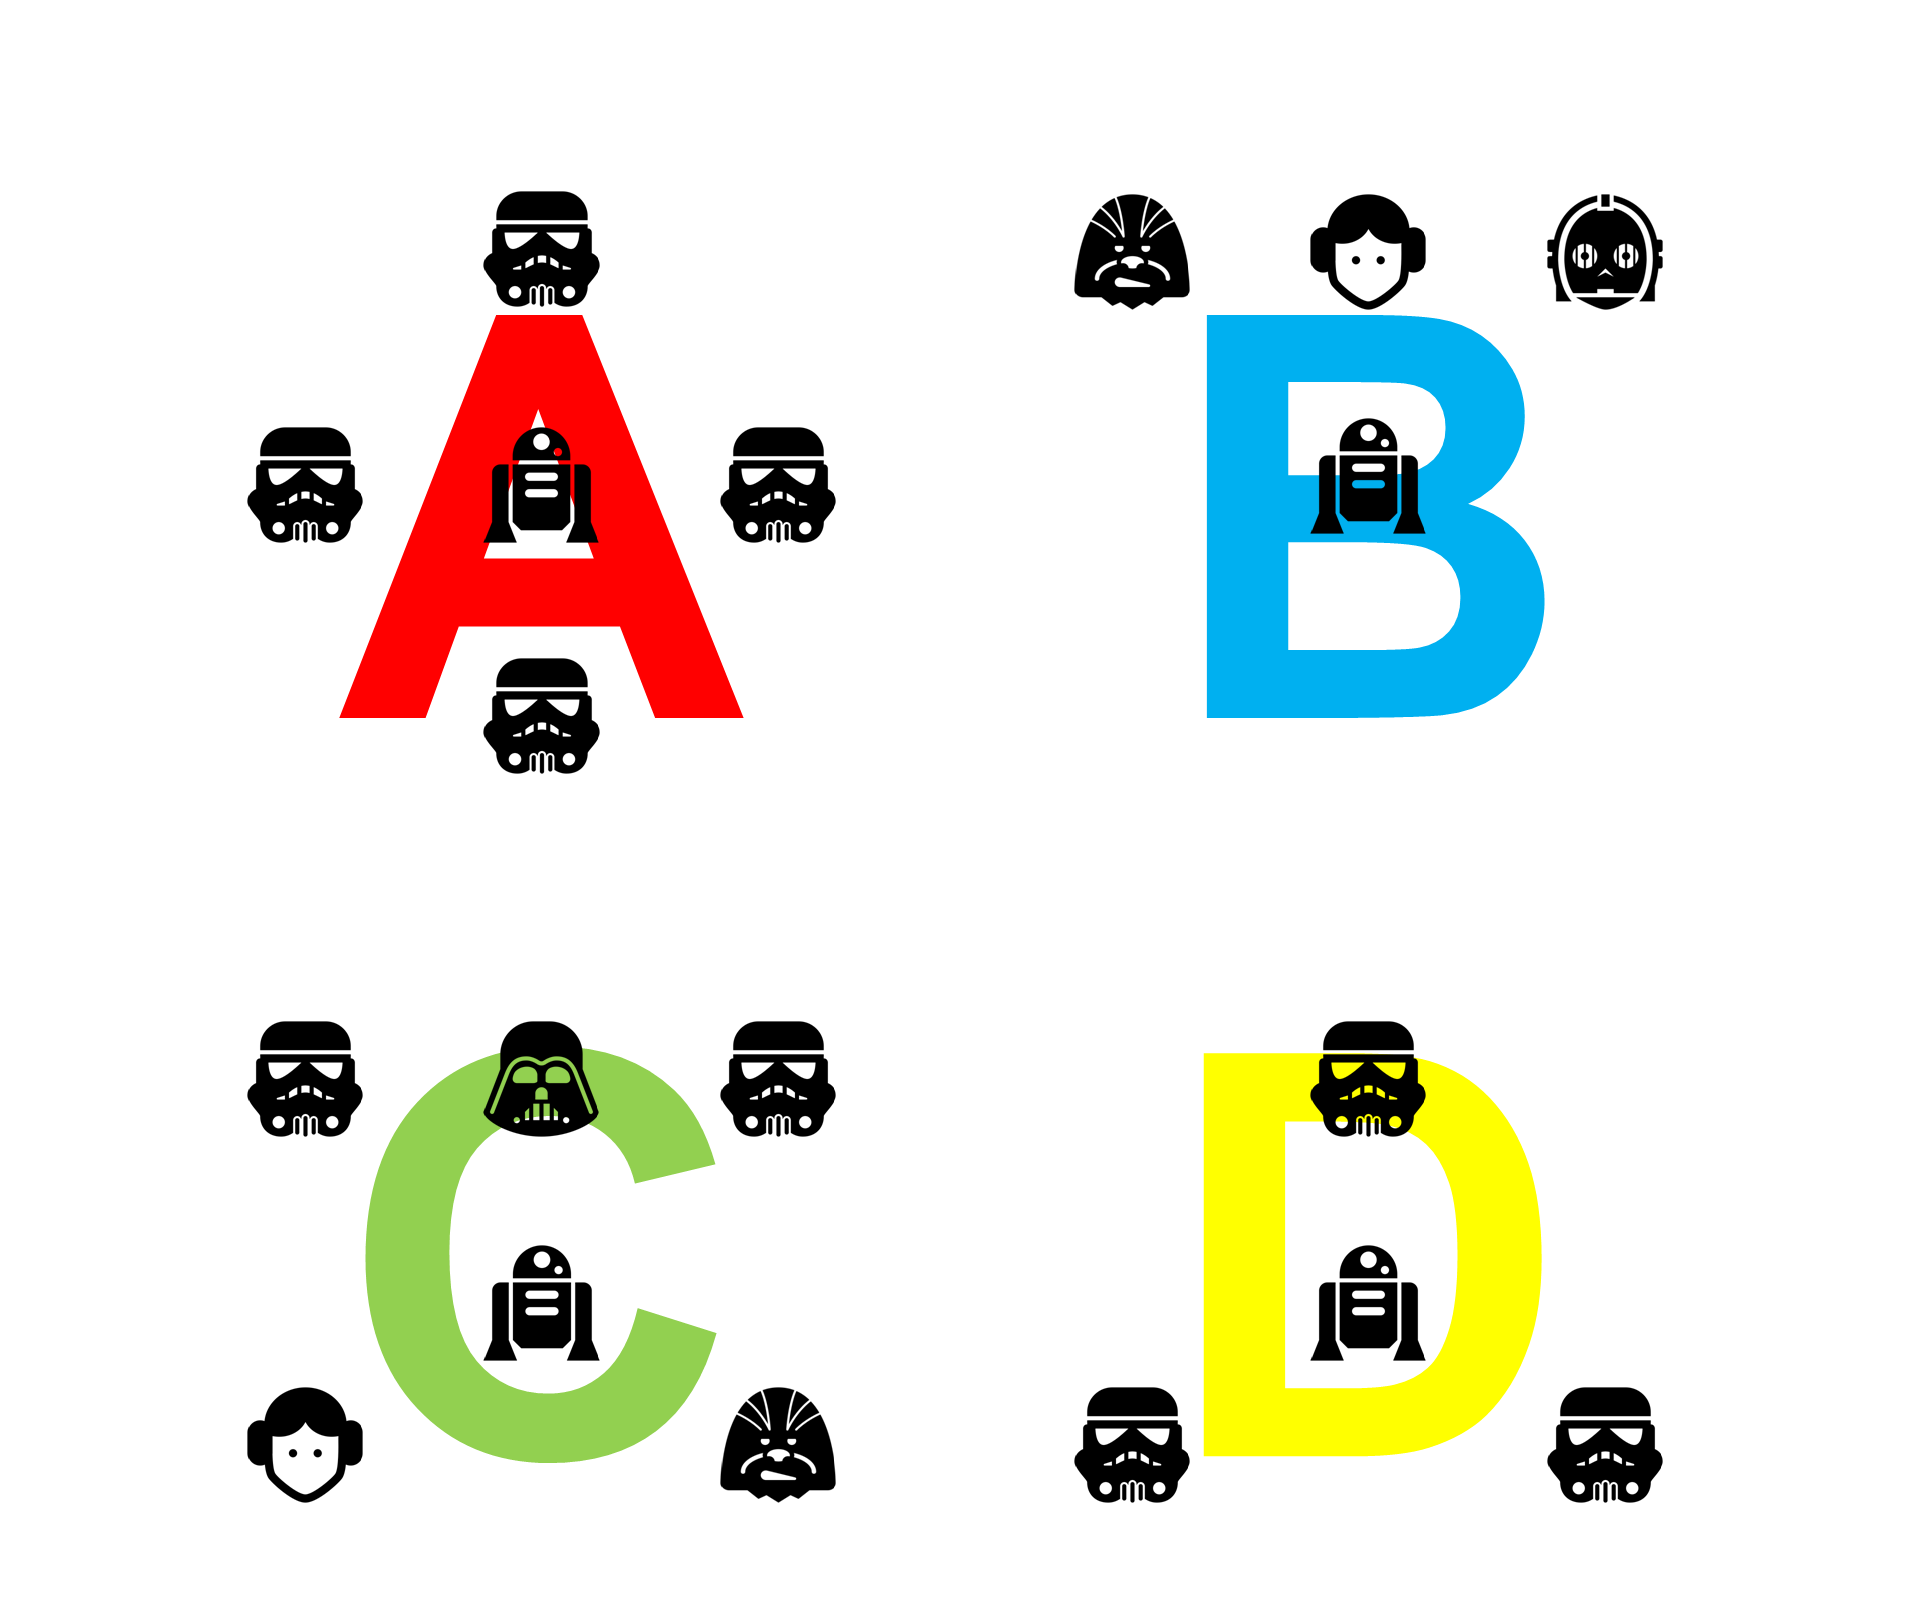
\includegraphics[width=0.75\textwidth]{images/spr_ppl_layout.png}
        \vspace{-10pt}
        \caption{Examples of people distribution in the \textit{blind man's bluff game}.}
        \label{fig:spr-ppl-layout}
    \end{center}
\end{figure}

% \begin{wrapfigure}[21]{r}{0.30\textwidth}
%     \vspace{-30pt}
%     \begin{center}
%         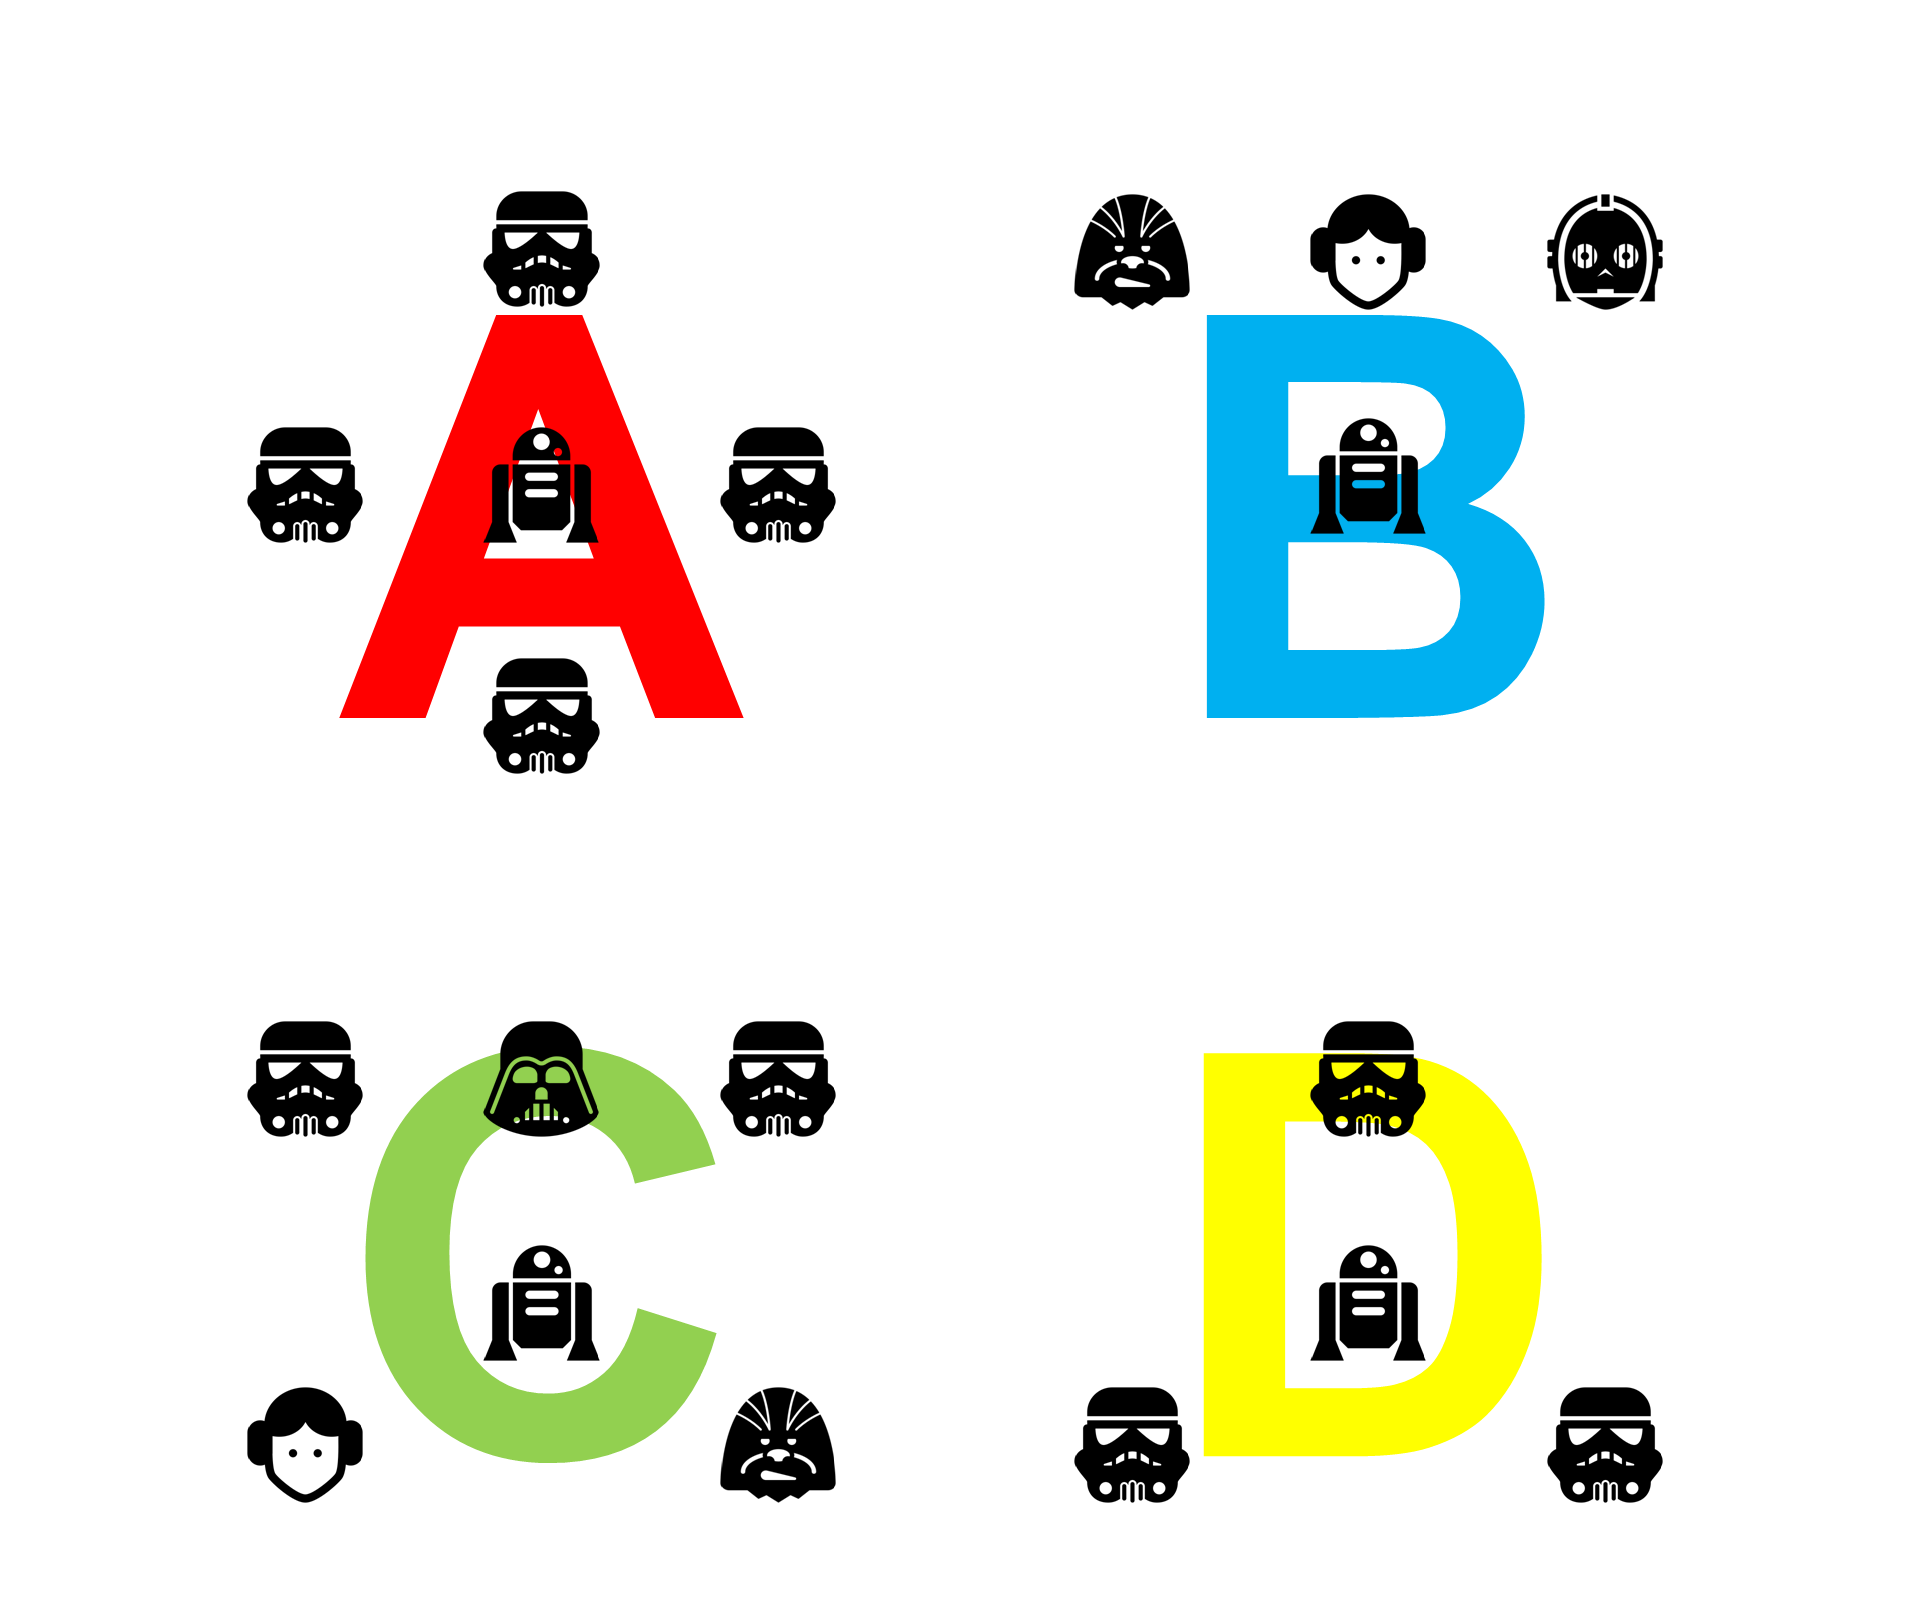
\includegraphics[width=0.25\textwidth]{images/spr_ppl_layout.png}
%         \label{fig:spr-ppl-layout}
%         \vspace{-10pt}
%         \caption{Examples of people distribution in the \textit{blind man's bluff game}.}
%     \end{center}
% \end{wrapfigure}

\subsection{People layout in DSPL}
People arrangement for robots competing in the Domestic Standard Platform League will follow a layout similar to B in Figure \ref{fig:spr-ppl-layout}; however, the number of people can vary.

Please note that after each question people will stay in place and proceed with the game without awaiting for the robot to reposition. This means that people might not be standing anymore facing the robot after it has turned. Also, since the people arrangement is linear, the distance between the robot and the spoken person can be larger than 1 meter.

\subsection{People layout in OPL}
People arrangement for robots competing in the Open Platform League will follow a layout similar to C in Figure \ref{fig:spr-ppl-layout}; although, the number of people can vary, all of them will be initially encircling and facing the robot. In this layout no person is allowed to be standing straight behind the robot, but slightly to the left or to the right.

Please note that after each question people will stay in place and proceed with the game without awaiting for the robot to reposition. This means that people might be standing straight behind the robot after it has turned. Also, although the referee will try to keep an even distance between the robot and the people, depending on the crowd size the 1 meter limit can be exceeded.

\subsection{People layout in SSPL}
People arrangement for robots competing in the Social Standard Platform League can follow a layout similar to either B or C in Figure \ref{fig:spr-ppl-layout}, but the number of people can vary.

In B-like (linear) layouts, since the people arrangement is linear, the distance between the robot and the spoken person can be larger than 1 meter.

Regarding C-like (circular) layouts all of them will be initially encircling and facing the robot. In this layout no person is allowed to be standing straight behind the robot, but slightly to the left or to the right.

Please note that after each question people will stay in place and proceed with the game without awaiting for the robot to reposition. This means that people might be standing straight behind the robot after it has turned, or beyond the 1 meter limit.